\section{Streaming Discharging Algorithm}
In this section we introduce stream discharging algorithm for CP, SED, DFA,
and informally motivate the features we need from the underlying
proof system. We discuss how lookup arguments (both internal and external)
are used to construct proofs for relational database operations.

We first given an informal overview below.
Consider a sample $s$ to be discharged of a collection of regex 
$\{r_i\}_{i=1}^n$. In many cases, due to circuit size restriction,
we have to chunk $s$ into many chunks 
$s = s^{(1)} \concat ... \concat s^{(k)}$, and run
``streaming" version of CP, SED, DFA over the chunks and combine
the results.

The design for streaming DFA or CP is straigh-forward. Essentially
we walk $s$ through the (AC)-DFA compiled from the regex set.
At each step of folding, we run a chunk $s^{(j)}$ over the DFA.
Then we need to pass the last state of the acceptance path as the
initial state for the next folding step. 
For SED algorithm, streaming is much more complex. We need to 
maintain the state of the ``step queue" for each subsignature, 
i.e., the list of occurene locations for each step of each step queue.
We need to perform forward and backward pruning at each folding stage
to minimize the size of the step queue, and between steps,
we need to pass the output ``step queue" to the next stage.
This step queue is huge, and it can only used for one time.
We need a concretely efficient way to pass large data structures
in between the neighboring steps of folding.

In summary, at each step of folding we run a ``streaming" (chunked)
version of CP, SED, DFA as follows:
\begin{enumerate} 
\item The prover first run a planning algorithm to determine 
the set of signatures to be discharged by each of CP, SED, DFA, and
ISED. Each algorithm is modeled as a separate gadget circuit,
and conditionallyl include them only when then are needed. For instance,
for most binary samples, only CP and SED are included, and very rarely
DFA or ISED would be needed.
\item At each step of folding, the circuit drives CP, SED, DFA, and ISED
(if included) concurrently. Mainly walking through the (AC)-DFA of each
method, passing needed data in between the neighboring steps.
\item At the last chunk for the word sample to discharge, the circuit
includes an additional component to compute the signatures that
cannot be discharged by CP (i.e., the signatures mapped from the
accepting state of the corresponding AC-DFA). Similarly, the signature
discharged by DFA is produced. For SED and ISED, it examines the
step queue of each subsignature, decide their tri-logic value and
run the boolean formula of subisngatures to determine the tri-logic
value of signatures and produce the discharge list of signatures.
Then it asserts that the union of SED, DFA, ISED discharged signatures
is equal to the set that cannot be discharged by CP. This completes
the assertion of $s$ free of regex signature set.
\end{enumerate}

\begin{figure*}[t!]
	\centering
	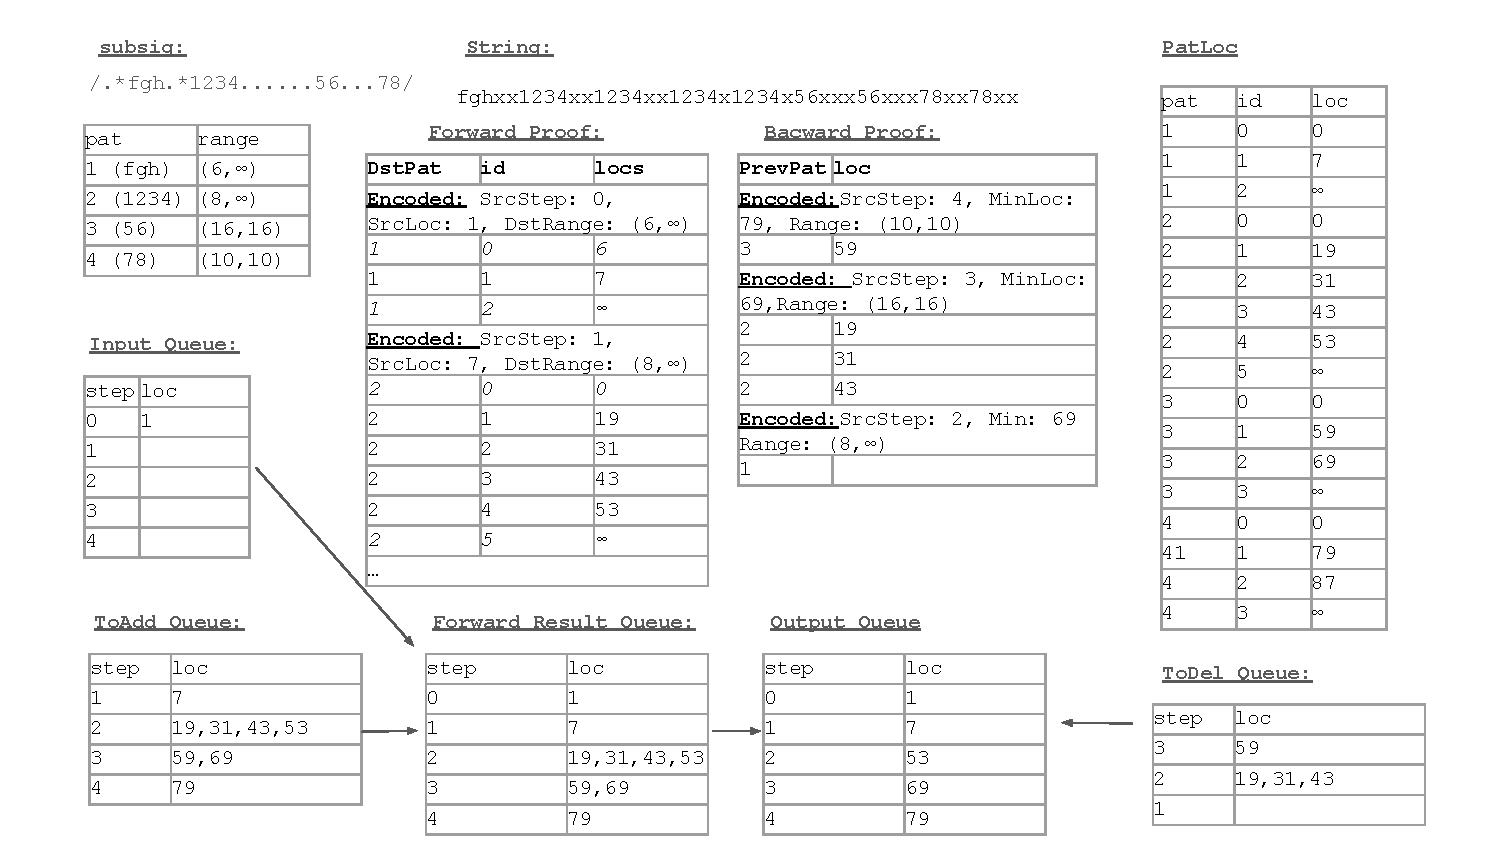
\includegraphics[width=\textwidth]{figs/FwdBwd.pdf}
\caption{Streaming Workflow for Foward and Backward Pruning}
\label{fig_stream}
\end{figure*}

\subsection{Streaming Algorithm for SED}
We now present the streaming algorithm for SED. We show how to use
internal lookups to support relational database operations needed.

We start with an informal introduction and a motivating example.
Recall that SED tries to discharge a string $s$ against 
a regex subsignature $r$ by checking the distance between patterns
of $r$. In Figure \ref{fig_stream}, we show an example
of regex which consists of four patterns (``fgh", ``1234", ``56", and ``78"). 
Each pattern has an expected range of distance from the match of
a previous pattern. For instance, the distance between ``1234" and ``56"
should be 16 nibbles (i.e., 8 characters, because the length of ``56"
is also counted).

SED has a pre-compiled AC-DFA that corresponds to all these patterns.
Before running the forward-backward pruning algorithm, SED feeds
the given string to the ACDFA, gets the list of final states,
and then map these final states back to the corresponding pattern words.
As an example, the word ``fghxx1234..." in Figure \ref{fig_stream}
generates the ``PatLoc" table as shown. For instance, one can see
that pattern 2 occurs at locations (9, 13, 43, 53). Note that
the first location starts from 1, and each location accounts for one 
4-bit nibble.

Then SED maintains a StepQueue that records the list of locations
that correspond to each pattern (step) in the regex subsignature.
For instance, given the regex signature and input word in Figure \ref{fig_stream}, starting with an initial input queue (where location 1 for step 0
is included by default), it results in the Output Queue as shown 
in the figure.

The challenge of making the prover more eficient is that: we need
to eliminate those ``dead" locations from the step queue at run time.
We thus develop a forward-backward pruning algorithm. Consider the
following example.

\begin{example}
	Given the example in Figure\ \ref{fig_stream}. The forward process
first iteratively starts from each location of each step, identify
the applicable locations for the next step. For instance, given location 7
for step 1 (pattern 7), four locations of the next pattern (2) falls
into the range (within min-max distance (16,16): 19, 31, 43, 53.
Notice that the algorithm has to roll based on the ``on-going" result.
For step 3, it has to start from the newly generated locations (19, 31, 43, 53),
and identify the workable locations 59 and 69 for step 3 and so on.

   Once the forward process is done, we then run a backward pruning process
that removes ``dead" locations. Consider step 4, its current minimum
location is 79. Given that the distance between step 3 and 4 is 10,
this eliminates $59$ in step 3, because for new locations for step 4
added in the future, they can only be greater than 79 and for sure
there will be no new locations that can be derived from 59. Thus
59 should be removed from the location list of step 3. Similalry,
the new ``min-loc" for step 3 now becomes 69, and this eliminates
19, 31, 43 from step 2. The list to delete is shown in ``ToDel Queue"
in Figure \ref{fig_stream}, which results in the final Output Queue.
\end{example}
